
\section{Relação Tempo-Frequência}
    
    \subsection{Contexto}
        Para o caso real, os sinais de áudio convoluem com a resposta ao impulso de um filtro, que representa o percurso realizado pelos mesmos entre as fontes e os sensores. Isto caracteriza um caso de misturas convolutivas (conforme visto na seção [referência]). 
        
        Com o conhecimento de que podemos representar uma operação de convolução no domínio tempo da mesma forma do que uma multiplicação no domínio da frequência, uma forma de simplificar este problema seria aplicar a transformada de Fourier à estes sinais, resolver múltiplos casos de misturas instântaneas e aplicar a transformada inversa de Fourier para levar os sinais de volta ao domínio do tempo. Uma das vantagens desta abordagem reside na redução da complexidade computacional e qualquer algoritimo ICA que trabalhe com números complexos e misturas instantâneas está apto para ser usado.
        
        Entretanto, as ambiguidades de escalamento e permutação inerentes ao problema de BSS (Seção [~\href{cap1}]), se tornam elementos centrais no processo de separação e precisam ser resolvidas. Ao trabalhar no domínio da frequência, a ICA fornece componentes independentes em cada raia de frequência, mas as as componentes de cada fonte não forem devidamente agrupadas antes de serem levadas para o domínio do tempo novamente. Isto é crucial para obter uma solução aceitável.
        
        Também é relevante citar o problema da circularidade da DFT. No caso discreto, o produto no domínio da frequência corresponde à convolução circular no domínio do tempo. Isto restringe o caso em que os filtros no domínio do tempo sejam periódicos, o que não é condizente com a realidade. Para fazer com que a multiplicação no domínio da frequência seja equivalente à convolução linear no domínio do tempo, é necessário que a representação do sinal no domínio do tempo deve ter um número de raias de frequência maior ou igual ao tamanho do filtro somado ao trecho do sinal, além do sinal ter de ser reconstruído através da técnica de Overlap-Add [referência]. Este processo é conhecido como \textit{FFT Filtering} e é amplamente utilizada para realizar convolução rápida de um filtro com um sinal longo. Quando isto não é respeitado, o sinal provinente do tratamento na frequência, seguido da sua IDFT será uma versão distorcida do sinal equivalente à convolução no domínio do tempo.
    
    \subsection{Sumário}
        O processo de tratamento do problema de FDBSS está ilustrado na Figura ~\ref{fig:frequencymodel} e pode ser estruturado da seguinte forma:
        
        \begin{enumerate}
            \item Inicialmente, transforma-se os vetores de misturas $\mathpzc{x_j}(n)$, j = 1,$\dots$,M em suas representações no domínio da frequência $\mathpzc{x_j}(m,k)$ , k = 0, $\dots$, K-1 (sendo \texit{m} o índice do \textit{frame} e K o número de raias de frequência), através da \textit{STFT}
            
            \item Como uma etapa de pré-processamento, realiza-se um branqueamento nos sinais, obtendo-se os sinais branqueados no domínio da frequência  $\mathpzc{z_j}(m,k)$ e a matriz branqueadora $\mathcal{V}$($\mathpzc{k}$).
            
            \item A etapa de processamento, que consiste na separação propriamente dita, é realizada, gerando uma matriz separadora $\mathcal{W}$($\mathpzc{k}$) para cada raia de frequência \texit{k}, além do vetor com as saídas separadas $\mathbf{y}$($\mathpzc{m,k})$ = [$\mathpzc{y_1}$($\mathpzc{m,k})$, $\dots$, $\mathpzc{y_N}$($\mathpzc{m,k})$]$^T$, sendo que tanto este quanto aquela estão fora de ordem e de magnitude.
            
            \item Já como um pós-processamento, são resolvidas as questões de permutação e escalamento, através das matries $\mathcal{P}$($\mathpzc{k})$ e $\Lambda$($\mathpzc{k})$.
            
            \item Por fim, é necessário levar o vetor com as saídas separadas novamente para o domínio do tempo através da \textit{ISTFT}.
            
        \end{enumerate}

        \begin{figure}[h!]
            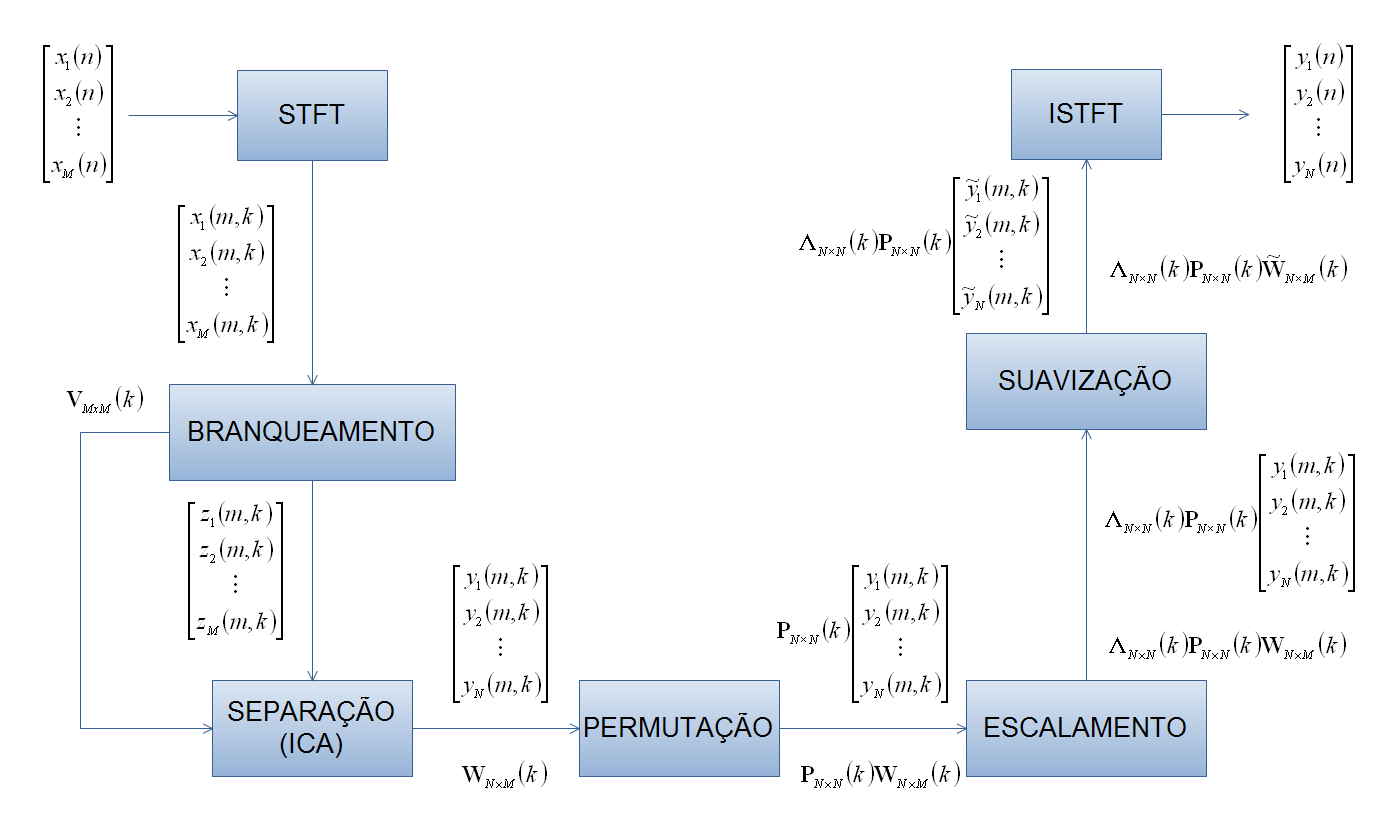
\includegraphics[scale=0.4]{frequencyprocess.png}
            \caption{Esquema do processo de FDBSS.}
            \label{fig:frequencymodel}
        \end{figure}

    \subsection{STFT}
        A STFT de um sinal x é dada pela equação abaixo (\ref{eq:STFT}), onde:

    %STFT
    \begin{equation}\label{eq:STFT}
        \mathcal{X}(\mathpzc{m},\mathpzc{k})
        = \sum_{n} \mathbf{x}(\mathpzc{n})
        \mathpzc{win}_\mathpzc{a}(\mathpzc{n} - \mathpzc{mJ})
        exp \left( -j \frac{2\pi\mathpzc{kn}}{K} \right), \mathpzc{k} = 0, \dots, K-1
    \end{equation}


        \begin{itemize}
            
            \item \mathpzc{k} é a raia de frequência, com intervalo [0, K-1]. Pode ser interpretada como a frequência discreta $\mathpzc{f_k}$ $\in$ \big\{0,$\frac{1}{K}$ $\mathpzc{f_s}$, \dots, $\frac{K-1}{K}$ $\mathpzc{f_s}$ \big\}.
                        
            \item K é o número de raias de frequência da DFT.
                        
            \item L é o comprimento da janela.
                        
            \item J é o deslocamento da janela.
            
            \item  $\mathpzc{f_s}$ é a frequência de amostragem.
            
            \item $\mathpzc{win_a}$($\mathpzc{n}$) é a janela de análise, definida como sendo não-nula apenas no intervalo [0, L-1]. O salto J é obviamente menor ou igual L, ou haverá perda de observações. Este saldo deve ser bem escolhido para não haver distorções na síntese dos sinais.
        \end{itemize}
    
        Pode-se notar que K=L na equação acima. Entretanto, há casos em que K$>$L, que são chamados de \textit{oversampled}. Nestes casos, é necessário fazer \textit{zero-padding} para preencher o sinal com zeros antes de passar para a frequência, conforme descrito em (\cite{STFT})
        
        A notação prática do cálculo da STFT está em (~\ref{eq:practiceSTFT}), onde:


        \begin{equation}\label{eq:practiceSTFT}
            \mathcal{X}(\mathpzc{m})
            = DFT(diag(\mathbf{x_{frame}}(\mathpzc{m})\mathbf{win_a}))
         \end{equation}
    
        \begin{enumerate}
        
            \item $\mathbf{DFT(v)}$ representa a DFT do vetor $\mathbf{v}$, que pode ser calculada através da FFT.
            
            \item O vetor $\mathbf{x_{frame}}$(m) = [$\mathpzc{x}$($\mathpzc{mJ}$), $\dots$, $\mathpzc{x(mJ + L - 1)}$]$^T$ tem comprimento L e representa o \textit{frame m} no domínio do tempo
            
            \item O vetor $\mathcal{X}(\mathpzc{m})$ = [$\mathcal{X}$($\mathpzc{f_0,m})$, $\dots$, $\mathcal{X}$($\mathpzc{f_{K-1},m}$)]$^T$ tem comprimento K e é o vetor com a representação em
            frequência do \texit{frame m}.
            
            \item O vetor $\mathbf{win_a}$ contém os elementos não nulos da janela mostrada em ~\ref{eq:STFT}. Assim sendo, tem comprimento L. O produto diag($\mathbf{x}$($\mathpzc{mJ}$))$\mathbf{win_a}$ resulta em um vetor de comprimento L. Por conta disos, se K $>$ L, devem ser realizado um \texit{zero-padding} de K - L amostras no final do vetor antes de aplicar a DFT.
        
        \end{enumerate}
        A notação prática do cálculo da ISTFT está em (~\ref{eq:practiceISTFT}) e (~\ref{eq:practiceISTFT2})
        
        \begin{equation}\label{eq:practiceISTFT}
            \mathbf{y_{frame}}(\mathpzc{m})
            = diag(\mathbf{win_s}IDFT(\mathcal{Y}(\mathpzc{m}))
         \end{equation}
        
        \begin{equation}\label{eq:practiceISTFT2}
            \mathbf{y}(\mathpzc{n})
            = \sum_{m}SHIFT(\mathbf{y_{frame}}(\mathpzc{m}),\mathpzc{mJ},\mathbf{N_{amost}})
         \end{equation}
        
        O sinal $\mathbf{y}$($\mathpzc{n}$) tem o comprimento de $N_{amost}$ e a operação SHIFT($\mathbf{a}$,b,c) desloca o vetor $\mathbf{a}$ de b amostras e aumenta seu comprimento para c, de forma que o vetor resultante tenha P elementos não-nulos, onde P é o tamanho do vetor $\mathbf{a}$.
        
        A técnica de \textit{Overlap-Add} consiste em acrescentar \textit{frames} superpostos para formar o sinal completo novamente. Também conhecida como OLA, esta técnica possui algumas variações, tais como a WOLA (\textit{Weighted Overlap-Add}) e a COLA (\textit{Constant Overlap-Add}). Esta técnica utiliza-se de uma janela de síntese $\mathpzc{win_s}(n)$ para a realização da ISTFT. Relacionar a janela de síntese $\mathpzc{win_s}(n)$ com a janela de análise $\mathpzc{win_a}(n)$ e os tamanhos dos comprimentos das janelas e dos sinais é fundamental para criar condições para que a transformação de volta para o domínio do tempo não possua distorções. 
        
        Para que a \textit{FFT Filtering} (necessária para resolver o problema de produto no domínio de  frequência discreta ser equivalente à convolução circular no domínio do tempo) gere um resultado satisfatório, as condições (\ref{eq:condition1}) e (\ref{eq:condition2}) devem ser satisfeitas. A condição (\ref{eq:condition2}) é chamada de condição COLA. Se não houver transformação ou a transformação for não-linear, a condição passa a ser (\ref{eq:condition3}). 
        
        \begin{equation}\label{eq:condition1}
            K \geq L + Q - 1
        \end{equation}
        
        \begin{equation}\label{eq:condition2}
            \sum_m \mathpzc{win_a(n - mJ) = c , c} constante, \forall\mathpzc{n} \in \mathbb{Z}
        \end{equation}
        
        \begin{equation}\label{eq:condition3}
            \sum_m \mathpzc{win_a(n - mJ)}\mathpzc{win_s(n - mJ) = c , c} constante, \forall\mathpzc{n} \in \mathbb{Z}
        \end{equation}
        
        
        Neste trabalho, iremos utilizar a janela de \texit{Hanning} (\ref{eq:hanning}) como janela de análise, atendendo à condição COLA (\ref{eq:condition2}). Para isto, usaremos J = $\frac{L}{2}$. Normalmente, a janela retangular é escolhida como a janela de síntese. Existem estudos acerca da utilização de outras janelas e em quais condições estas satisfazem ou não a COLA. Recomendamos a leitura de \cite{LuizVictorio} para maior aprofundamento no assunto.
        
        \begin{equation}\label{eq:hanning}
            \mathpzc{w_{hanning}(n)} = 0,5 \left( 1 - cos\frac{2\pi\mathpzc{n}}{L}\right)
        \end{equation}
        
\section{Pré-Processamento}
    O estágio de pré-processamento pode surgir de três formas: necessário, auxiliar ou desnecessário, dependendo do método de separação a ser empregado no processamento propriamente dito. O método mais comum de pré-processamento é o de \textit{branqueamento}, que se baseia na média do vetor de amostras.
    
    \subsection{Branqueamento}
        Em geral, branquear os vetores é uma boa prática, visto que faz grande parte do trabalho de separação, a descorrelação. Dependendo do método utilizado na etapa de separação, o branqueamento pode ser obrigatório (\textit{FastICA}) ou melhorar a velocidade e robustez da convergência do algoritmo ICA no domínio da frequência (\textit{Natural ICA}). A normalização do vetor de misturas desempenha um papel importante em sinais de áudio devido à sua característica de não-brancura (ou colorido), ou seja, a energia varia bastante entre as frequências.
        
        Matematicamente, é possivel mostrar que o processo de branqueamento faz aproximadamente metade do trabalho de separação, sem muito custo computacional. Entre outros benefícios, estão a rapidez e uniformidade na convergência para cada raia de frequência, quando utilizado um passo de adaptação fixo, além de ser pré-requistio dos algoritmos \textit{FastICA}.
        
        O processo é dividido em duas partes: A primeira consiste em fazer a centralização do vetor de misturas, isto é, fazer com que cada mistura possua média igual a zero. Feito isso, é necessário tornar a sua matriz de covariância igual à matriz identidade, resultando na descorrelação das componentes do vetor de amostras.
        
        A centralização pode ser realizada individualmente sobre cada uma das raias de frequência do vetor de amostras no domínio da frequência $\mathpzc{x_{jk}}(m)$, de forma a obter $\mathpzc{x_{jk}}(m)$ $\leftarrow$ $\mathpzc{x_{jk}}(m)$ - $\mathpzc{E}$$\{$$\mathpzc{x_{jk}(m)}$$\}$.
        
        Uma vez feita a centralização, tem-se que $\mathpzc{E}$$\{$$\mathbf{x}$$\}$ = 0 . Assim sendo, a matriz de covariância do vetor de misturas é dada por:
        
        \begin{equation}\label{eq:covariance}
            \mathbf{R_x} = \mathpzc{E}\{\mathbf{xx^T}\}
        \end{equation}
        
        O branqueamento se dá sobre cada frequência por uma matriz \mathbf{V}:
        
        \begin{equation}\label{eq:whiteningfrequency}
            \mathbf{z} = \mathbf{V}\mathbf{x}
        \end{equation}
        
        Para obtermos o vetor $\mathbf{z}$ com as suas componentes descorrelacionadas, precisamos encontrar a matriz branqueadora $\mathbf{V}$ tal que $\mathpf{R_z}$ = $\mathbf{I}$.

        \begin{equation}
            \label{whiteningproof}
        \mathpzc{R_z} = \mathbf{V}\mathbf{R_x}\mathbf{V^T} = I 
        \end{equation}

        Solucionando a equação acima em função de $\mathbf{V}$, chegamos à conclusão:
        
        \begin{equation}\label{eq:vk}
            \mathbf{V} = \mathbf{D}^{-\frac{1}{2}}\mathbf{E^T}
        \end{equation}
        
        A matriz $\mathbf{E}$ é a matriz que contém os autoetores da matriz de correlação $\mathbf{R_x}$, onde cada coluna é um autovetor e e $\mathbf{D}$ é uma matriz diagonal que contém os autovalores de $\mathbf{R_x}$. O resultado interessante é que se perumtarmos as matrizes $\mathbf{D}$ e $\mathbf{E}$, o produto $\mathbf{D}^{-\frac{1}{2}}\mathbf{E^T}$ se mantém, contanto que a permutação aplicada seja igual nas duas matrizes.
        
        Este resultado diz que podemos manipular as matrizes $\mathbf{D}$ e $\mathbf{E}$ de forma que o autovetor corresponda ao seu autovalor. Isto implica diretamente na redução dimensional do problema, uma vez que as componentes princiais do vetor de misturas corresponderão às primeiras linhas do vetor branqueado. Esta redução dimensional é conhecido como Análise de Componentes Principais (PCA), do qual surgiu o conceito de ICA. 
        
\section{Processamento}

    \subsection{Separação por Natural ICA}
    A separação dos sinais é realizada em cada raia de frequência, utilizando um algoritmo ICA que trabalhe com números complexos. O algoritmo Natural ICA, por não possuir restrições com relação à matriz separadora, é uma boa escolha.
    No Natural ICA, após o branqueamento das amostras, a matriz de branqueamento $\mathbf{V_K}$ é utilizada como solução inicial $\mathbf{W_k = V_k}$ e a matriz $\mathbf{W_k}$ é atualizada iterativamente, utilizando o algoritmo apresentado em \ref{eq:matrixrefresh}
    
    \subsection{Separação por JADE}
    Na Seção \ref{secondorder} apresentamos que as informações de estatísticas de segunda ordem podem ser úteis em um processo de branqueamento e pode ser feito por meio da diagonalização da matriz de correlação relativa ao vetor de misturas $\mathbf{x}$. A JADE (\textit{Joint Approximate Diagonalization of Eigenmatrices})\cite{JADE} é uma abordagem em BSS que leva em consideração informações de \textit{HOS} através de processos de diagonalização das entidades que contenham tais informações, como o tensor de cumultantes e a matriz de cumultantes associada ao vetor aleatório. Relembramos a definição de um cumultante de quarta ordem (utilizado pela JADE):
    
    \begin{equation}
        \label{cumJADE}
        \begin{split}
        \mathpzc{cum(z_1,z_2,\dots,z_p)} = \mathpzc{E}\{\mathpzc{z_1z_2z_3z_4}\} - \mathpzc{E}\{\mathpzc{z_1z_2}\}\mathpzc{E}\{\mathpzc{z_3z_4}\} & \\ - \mathpzc{E}\{\mathpzc{z_1z_3}\}\mathpzc{E}\{\mathpzc{z_2z_4}\} - \mathpzc{E}\{\mathpzc{z_1z_4}\}\mathpzc{E}\{\mathpzc{z_2z_3}\}    
        \end{split}
    \end{equation}
    
    A definição de uma estrutura semelhante à matriz de correlação necessita do conceito de tensor, que pode ser entendido como uma extrapolação do conceito de matriz, no sentido de que um tensor pode apresentar um número de  entradas maior do que dois. Neste contexto, define-se o tensor de cumulante como um conjunto de elementos, sendo
que o elemento $\mathbf{ijkl}$ é dado por $\matbpzc{cum(z_i, z_j, z_k, z_l)}$, e com $\matphzc{i,j,k,l}$ variando de 1 a p.
    Um outro conceito que utilizaremos é o de matriz de cumulante associada a um vetor aleatório $\mathbf{x}$ = [$\mathpzc{x_1}$, $\dots$,  $\mathpzc{x_N}$] e a uma matriz M de dimensão N x N. No caso, o elemento ij da matriz de cumulante é dado por
    
    \begin{equation}
        \mathbf{[Q^x(M)]_{ij}} = \sum_{k,l=1}^N Cum(\mathpzc{x_i,x_j,x_k,x_l)M_{kl}}
    \end{equation}
    
    sendo que os índices i e j variam de 1 a N. A matriz de cumulante $\mathbf{Q^x(M)}$ pode ser entendida como o resultado da aplicação do tensor de cumulante de $\mathbf{x}$ à matriz $\mathbf{M}$, ou seja, $\mathbf{Q^x(M)}$ = $\mathbf{T(M)}$, onde $\mathbf{T(\cdot)}$ representa a transformação efetuada por um tensor.
    
    Veremos como essas medidas são consideradas no problema de separação. No caso em que o vetor x representa os sinais misturados após um etapa de branqueamento \ref{secondorder}, é possível mostrar (Cardoso, 1999) que a matriz de cumulantes associada a $\mathbf{x}$ é dada por
    
    \begin{equation}
        \mathbf{[Q^x(M)]_{ij}} = \mathbf{U\Delta(M)U^T}
    \end{equation}
    
    Onde $\mathbf{U}$ é a matriz branqueadora ortogonal e  $\mathbf{\Delta(M)}$ é uma matriz ortogonal cujos parâmetros dependem de $\mathbf{M}$ e das curtoses das fontes.

    Obviamente, a matria $\mathbf{U}$ diagonaliza  $\mathbf{Q^x(M)}$. Assim, a diagonialização de $\mathbf{Q^x(M)}$ é uma abordagem possível para a recuperação das fontes.  A diagonalização da matriz de cumultante garante a identificação de $\mathbf{U}$ desde que haja, no máximo, uma fonte com curtose nula (restrição sobre fontes gaussianas) e que os autovalores de $\mathbf{Q^x(M)}$ sejam distintos (Cardoso & Souloumiac, 1993). Como não se tem essa informação à priori da matriz $\mathbf{U}$, é impossível estabelecer qualquer tipo de garantia sobre esses autovalores.
    Assim sendo, em vez de se realizar a diagonalização considerando apenas uma matriz de cumulante, adota-se um esquema de diagonalização conjunta de diferentes matrizes de cumulante, sendo cada uma delas definida por uma matriz $\mathbf{M_i}$. Dessa forma, a função custo a ser minimizada no algoritmo JADE é dada por
    
    \begin{equation}\label{eq:optimize}
        \mathbf{D(U)} = \sum_i \Omega(\mathbf{U^TQ^X(M_i)U})
    \end{equation}
    
    onde o operador $\Omega(\cdot)$ expressa a soma quadrática dos elementos que não estão na diagonal principal. Sobre a escolha das matrizes $\mathbf{M_i}$, escolhem-se automatrizes relativas ao tensor de cumulante, ou seja, as N matrizes $\mathbf{M_i}$ tal que $\mathbf{Q^x(M_i)}$ = $\lambda$ $\mathbf{M_i}$.
    
    O método de Jacobi para diagonalização de matrizes pode ser utilizado para otimizar a função \ref{eq:optimize}. A idéia essencial é representar a matriz $\mathbf{U}$ como um produto de matrizes de rotação
    
    \begin{equation}
        \mathbf{U} = \sum_{i,j=1,i\neqj}^N \mathbf{R_{ij}},
    \end{equation}
    
    onde a matriz de rotação $\mathbf{R_{ij}}$ , de dimensões N x N, é idêntica a uma matriz identidade, exceto seus elementos nas posições $\mathpzc{(i,i), (i,j), (j,i), (j,j)}$, que são dados por 
    
    \begin{equation}
        \mathpzc{r_{ii} = cos \theta, r_{ij} = sin \theta, r_{ji} = -sin \theta, r_{jj} = cos \theta}
    \end{equation}
    
    Onde $\theta$ é o ângulo de rotação. Em (Cardoso & Souloumiac, 1996) é proposta uma forma de determinar analiticamente qual o ângulo de rotação que minimiza a expressão [\ref{eq:optimize}]. A despeito do reduzido número de iterações necessárias para a convergência deste procedimento de diagonalização conjunta, tal técnica se torna consideravelmente ineficiente em cenários com um elevado número de fontes, devido ao aumento de complexidade presente na determinação analítica dos ângulos de rotação.
    
    Uma das razões pela qual o JADE é bastante atrativo é o fato de que tanto o desenvolvimento da função contraste [\ref{eq:optimize}], quanto o do processo de diagonalização conjunta são válidos para vetores aleatórios complexos (Cardoso & Souloumiac,1993). 
\section{Pós-Processamento}
    \subsection{Permutação}
    O principal desafio do ICA no domínio da frequência é o problema da permutação. Ele consiste em encontrar a matriz de permutação $\mathbf{P_k}$, definida na Seção \ref{sec:separability}, onde o índice $\mathpzc{k}$ indica a raia da frequência, de forma que se agrupe corretamente as frequências das fontes e a ISTFT gere resultados satisfatórios.
    Este problema pode ser tratado de diferentes maneiras, entretanto, para este trabalho, iremos destacar o método TDOA (\textit{Time Difference Of Arrival}), que pode ser considerado uma extensão do DOA (\textit{Difference Of Arrival}).
    
    O DOA se baseia no ângulo de chegada das fontes nos sensores. Entretanto, é possível que duas fontes tenham o mesmo DOA, devido a estimativa de DOA utilizada funciona em um plano 2D. Desta forma, fontes cujos ângulos de chegada tenham o mesmo valor de cosseno estão, para o algoritmo, na mesma posição. Isto cria uma uma limitação de ângulos entre 0 e 2$\pi$. Uma alternativa é estimar a posição num espaço tridimensional das fontes (DOA 3D), mas isto acarreta em um aumento significativo do custo computacional.
    
    O TDOA é uma alternativa mais robusta ao DOA. Baseando-se na diferença de tempos de chegada de cada fonte aos sensores, este não sofre a limitação de ângulo que o DOA sofre, além de não ser computacionalmente mais custoso. Através do TDOA de cada fonte entre todos os pares de sensores, é possível identificá-las em cada uma das raias de frequência.
    
    Ambos os métodos acima baseiam-se na idéia de estimar a localização das fontes através de informações sobre o sistema de mistura, além de classificar as fontes em cada raia de frequência baseado em sua localização.
    
    Baseado em \cite{LuizVictorio}, utilizaremos a abordagem do TDOA por mostrar um resultado satisfatório para o caso proposto. Novamente, convidamos o leitor interessado em se aprofundar nas diferenças entre os métodos para resolver permutação a consultar a referência.